\section{Results}

\label{sec:results}

\subsection{Model-selection context}

We retain \texttt{sensitiveai-vi-custom} as a focused, exploratory case study for
tracing decision provenance---a post-hoc analysis, not a confirmatory validation-based
selection. The strongest standalone backbone by validation macro-F1 is
\texttt{sensitiveai-vi-customdlr2stage} (70.89\%), also strongest on test (66.38\%), so
the fusion results are not evidence that the focused backbone is best standalone.

\subsection{The hybrid does not improve accuracy}

\label{sec:no-accuracy-gain}

Table~\ref{tab:fusion-variants} reports every variant. AI alone reaches 65.75\%
macro-F1 and 87.62\% accuracy; the per-channel hybrid reaches 66.02\% and 87.74\%, a gain
of 0.27\% and eight more correct comments (5{,}861 vs. 5{,}853), concentrated in
\hate{}: F1 rises 58.30\% to 59.06\% via recall (53.34\% to 54.94\%) at a small precision
cost (64.27\% to 63.85\%), while \off{} and \clean{} barely move.

Per-channel weights add 0.10\% over a global weight (65.83\% to 65.93\%), thresholds
a further 0.09\%. The logistic meta-classifier is worse than AI alone (65.13\%): six
features on 2{,}672 validation comments overfit. Thresholds make the rule engine
usable alone (52.58\% vs.\ 47.14\% with argmax).

\begin{table}[ht]
\centering
\scriptsize
\setlength{\tabcolsep}{3pt}
\caption{Decision-level variants for the focused backbone
(\model{sensitiveai-vi-custom}) on test. Every variant reads the same frozen
scores; only mixing and the decision rule differ; the last row is primary.
\emph{Per-class columns are F1 (in percent)}; best macro-F1 in bold. Rule-only rows are scored
inside the fusion pipeline on renormalised rule scores; the standalone engine with
its own thresholds is reported in the text.}
\label{tab:fusion-variants}
\begin{tabular}{lccccc}
\toprule
System & Acc. & Macro-F1 & \hate & \off & \clean \\
\midrule
AI only (argmax)                      & 87.62 & 65.75 & 58.30 & 44.93 & 94.03 \\
Rule only (argmax)                    & 84.94 & 47.14 & 48.67 & 0.00 & 92.74 \\
Rule only (frozen thresholds)         & 84.21 & 52.58 & 41.02 & 23.89 & 92.84 \\
\midrule
Fusion, global $\alpha$ (argmax)      & 87.69 & 65.83 & 58.51 & 44.90 & 94.08 \\
Fusion, global $\alpha$ (thresholds)  & 87.69 & 65.83 & 58.51 & 44.90 & 94.08 \\
Fusion, logistic meta-classifier      & 86.26 & 65.13 & 58.18 & 43.79 & 93.41 \\
Fusion, per-channel $\alpha$ (argmax) & 87.74 & 65.93 & 58.82 & 44.88 & 94.08 \\
Fusion, per-channel (thresholds)      & 87.74 & \textbf{66.02} & 59.06 & 44.94 & 94.07 \\
\bottomrule
\end{tabular}
\end{table}


Table~\ref{tab:precision-recall} gives precision and recall, overall (macro) and
per label. The hybrid's \hate{} gain is recall-driven (53.34\% to 54.94\%) at a small
precision cost (64.27\% to 63.85\%); macro precision rises 68.43\% to 68.74\% and macro
recall 63.59\% to 63.83\%.

\vspace{12pt}
\begin{table}[ht]
\centering
\scriptsize
\setlength{\tabcolsep}{2pt}
\caption{Precision and recall on test for the focused backbone
(\model{sensitiveai-vi-custom}), over the same eight systems as
Table~\ref{tab:fusion-variants}. Per-class columns are precision (P)
and recall (R) in percent; macro averages are unweighted means. Best value in
each column is bold. Different systems win different columns: the
logistic meta-classifier has the highest recall but the lowest
macro-F1 (Table~\ref{tab:fusion-variants}), which aggregate F1 hides.}
\label{tab:precision-recall}
\begin{tabular}{lcccccccc}
\toprule
System & \multicolumn{2}{c}{\hate} & \multicolumn{2}{c}{\off} & \multicolumn{2}{c}{\clean} & \multicolumn{2}{c}{Macro} \\
\cmidrule(lr){2-3}\cmidrule(lr){4-5}\cmidrule(lr){6-7}\cmidrule(lr){8-9}
 & P & R & P & R & P & R & P & R \\
\midrule
AI only (argmax) & 64.27 & 53.34 & 48.44 & 41.89 & 92.58 & 95.53 & 68.43/63.59 \\
Rule only (argmax) & 46.90 & 50.58 & 0.00 & 0.00 & 89.69 & \textbf{96.00} & 45.53/48.86 \\
Rule only (thresholds) & 62.50 & 30.52 & 23.48 & 24.32 & 90.19 & 95.66 & 58.72/50.17 \\
Fusion, global $\alpha$ (argmax) & 64.56 & 53.49 & 48.68 & 41.67 & 92.58 & 95.62 & 68.61/63.59 \\
Fusion, global $\alpha$ (thresholds) & 64.56 & 53.49 & 48.68 & 41.67 & 92.58 & 95.62 & 68.61/63.59 \\
Fusion, logistic meta-classifier & 53.47 & \textbf{63.81} & 45.61 & \textbf{42.12} & \textbf{94.26} & 92.57 & 64.45/\textbf{66.17} \\
Fusion, per-channel $\alpha$ (argmax) & \textbf{64.91} & 53.78 & 48.94 & 41.44 & 92.55 & 95.66 & \textbf{68.80}/63.63 \\
Fusion, per-channel (thresholds) & 63.85 & 54.94 & \textbf{49.73} & 40.99 & 92.64 & 95.55 & 68.74/63.83 \\
\bottomrule
\end{tabular}
\end{table}


\vspace{6pt}
\begin{figure}[ht]
\centering
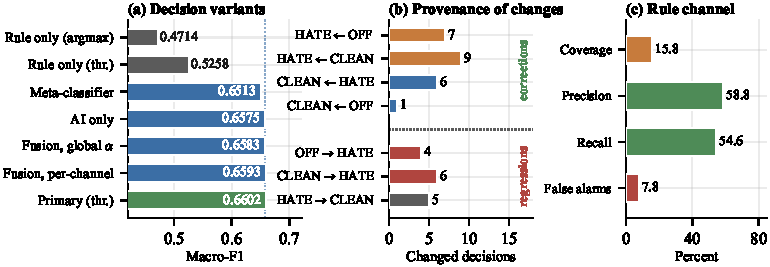
\includegraphics[width=0.85\textwidth]{figures/results.pdf}
\caption{Focused backbone. (a)\ Macro-F1 of each variant (dotted: AI-only).
(b)\ Provenance of the 38 changed decisions. (c)\ Rule-channel coverage, precision
when firing, recall on non-\clean{}, and false alarms on \clean{} (percentages).}
\label{fig:results}
\end{figure}

\subsection{The difference is not distinguishable from zero}

\label{sec:significance-results}

The negative result is explicit: for the focused
backbone the paired-bootstrap difference is $-0.27\%$ (95\% CI $[-0.79,+0.27]\%$,
$p=0.29$) and McNemar gives $b=15$, $c=23$, $p=0.26$. Every bootstrap interval
across the four backbones contains zero. Where McNemar reaches significance the sign
flips (standard head loses 61/wins 30, $p=0.0015$; curriculum loses 8/wins 31,
$p=0.0003$). The hybrid is \emph{accuracy-neutral}: 38 decisions change without
moving the aggregate metric beyond noise.

\subsection{The rule channel is narrow and precise}

\label{sec:rule-channel-results}

The rule engine fires on 1{,}052 of 6{,}680 comments (15.75\%) at 58.75\% precision,
recovers 54.59\% of non-\clean{} comments and fires on 7.82\% of \clean{} ones
(Fig.~\ref{fig:results}c): Signals from the Rule Engine serve to supplement the evidence available to the model, rather than independently determining the classification outcome. Coverage is low by
construction (multi-word, context-required phrases; validation zeroed the accent-less
alias weight), so it matches near-canonical forms.

\subsection{Leak-free sensitivity analysis}

\label{sec:leak-free-sensitivity}

With the 671-entry leak-free lexicon, the standalone rule engine reaches 53.98\%
validation and 53.28\% test macro-F1. Leak-free fusion obtains 5{,}863 correct
predictions, 23 corrections and 13 regressions (36 changes), macro-F1 66.12\%; the
canonical setup gives 5{,}861 correct, 23 corrections and 15 regressions (38 changes),
macro-F1 66.02\%. Separate sensitivity result, not the headline.